\subsection{Subgraph Isomorphism Proof}
\label{sec:SubgraphIsomorphismProof}


Suppose certain one graph $G^o$ is subgraph of $G^*$. Based the mapping relationship from Sec.\ref{sub:SeVNDesignFormulation}, there must be a bijection mapping between node of graph $G$ and graph $G^o$. The some node $v_i$ of graph $G$ if and only if map a node $v_i^o$ of graph $G^o$. According to schema of our heuristic algorithm, there must exist one edge or create one edge ($v^o_iv^o_j$) regardless of  there is not edge between node $v^o_i$ and node $v^o_j$ , which is corresponding to edge $v_iv_j$ of graph $G$. Consequently, there must be a bijection function of every edge $e$ of graph $G$ to edge $e^o$ of graph $G^o$, $G$ is isomorphic to graph $G^o$, graph $G^o$ is subgraph of $G^*$, $G$ is subgraph isomorphism of graph $G^*$





\begin{figure}
  \centering
  % Requires \usepackage{graphicx}
  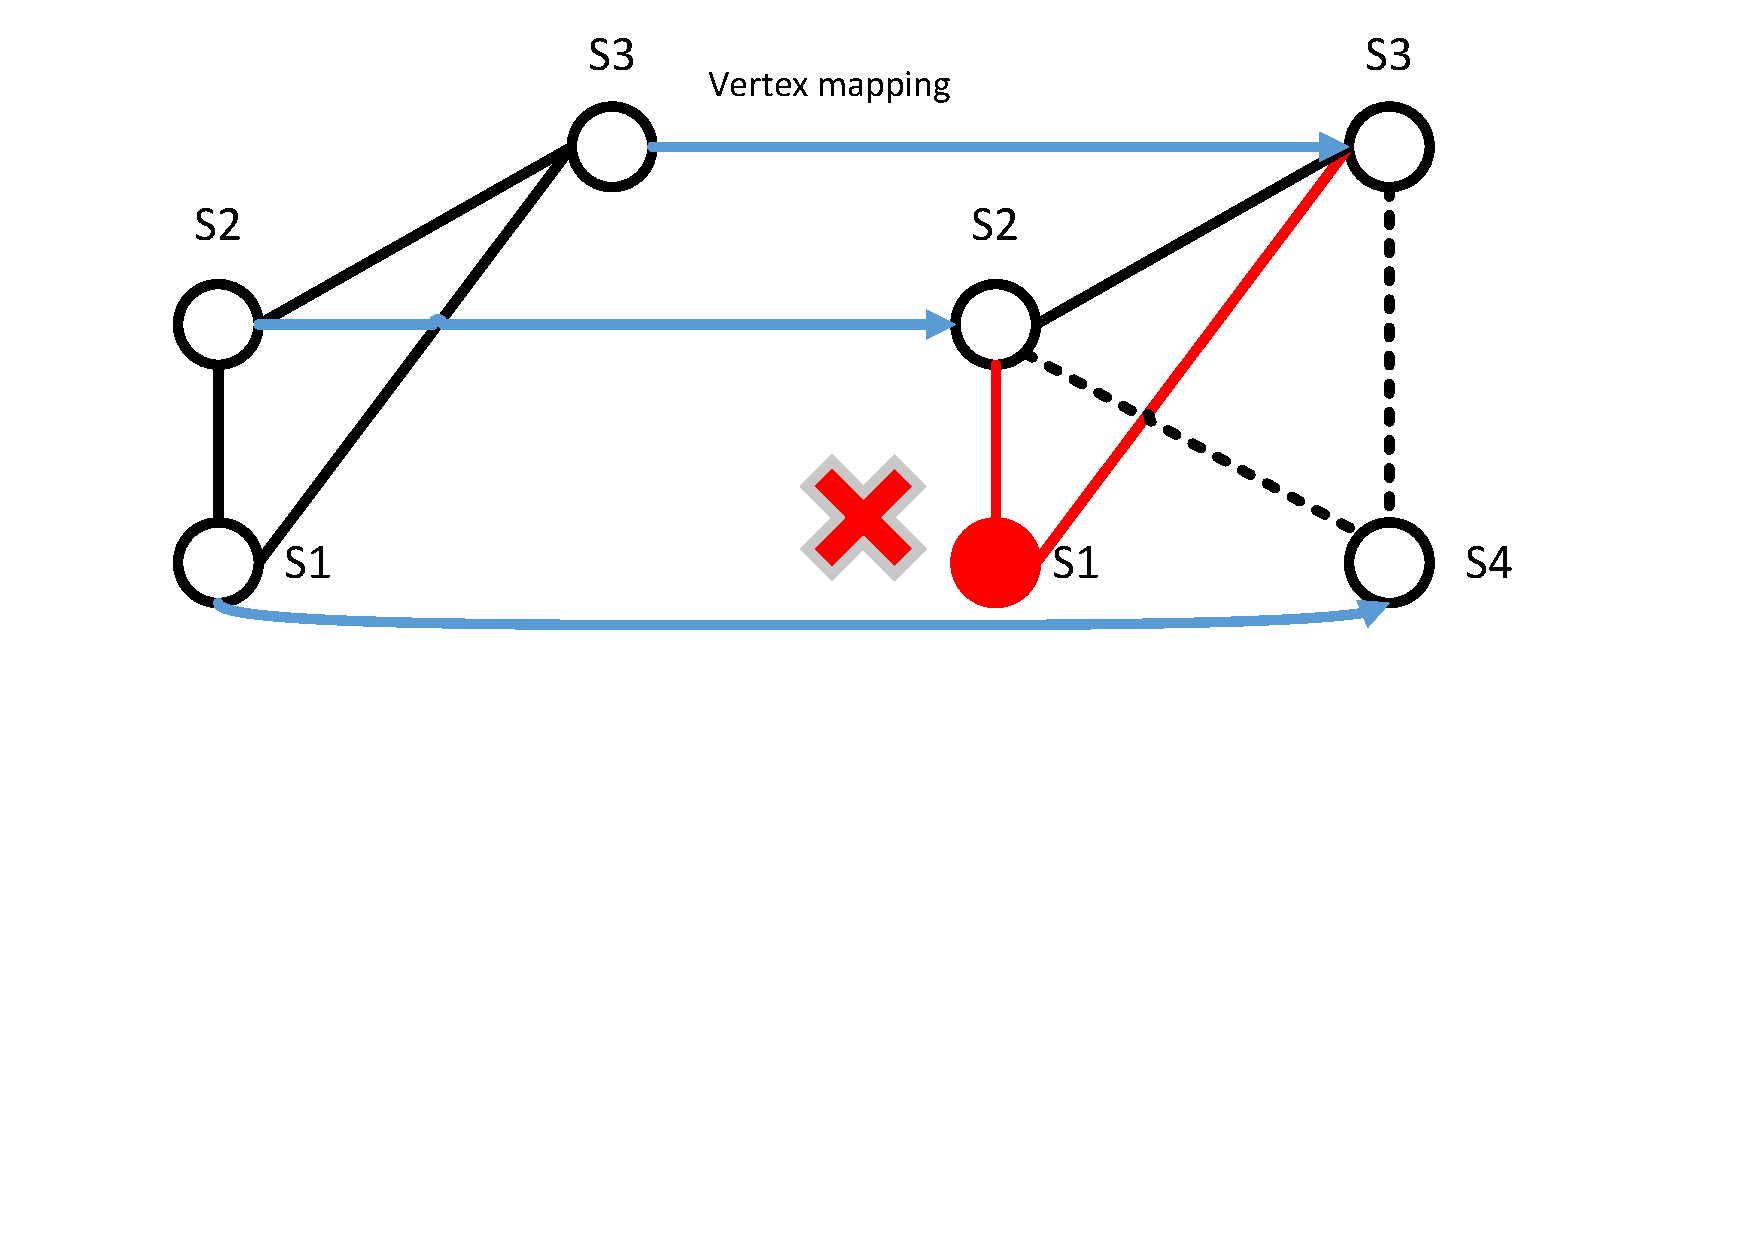
\includegraphics[width=1.5in]{Fig/MapA}\\
  \caption{MapA}\label{Fig:MapA}
\end{figure}

\begin{figure}
  \centering
  % Requires \usepackage{graphicx}
  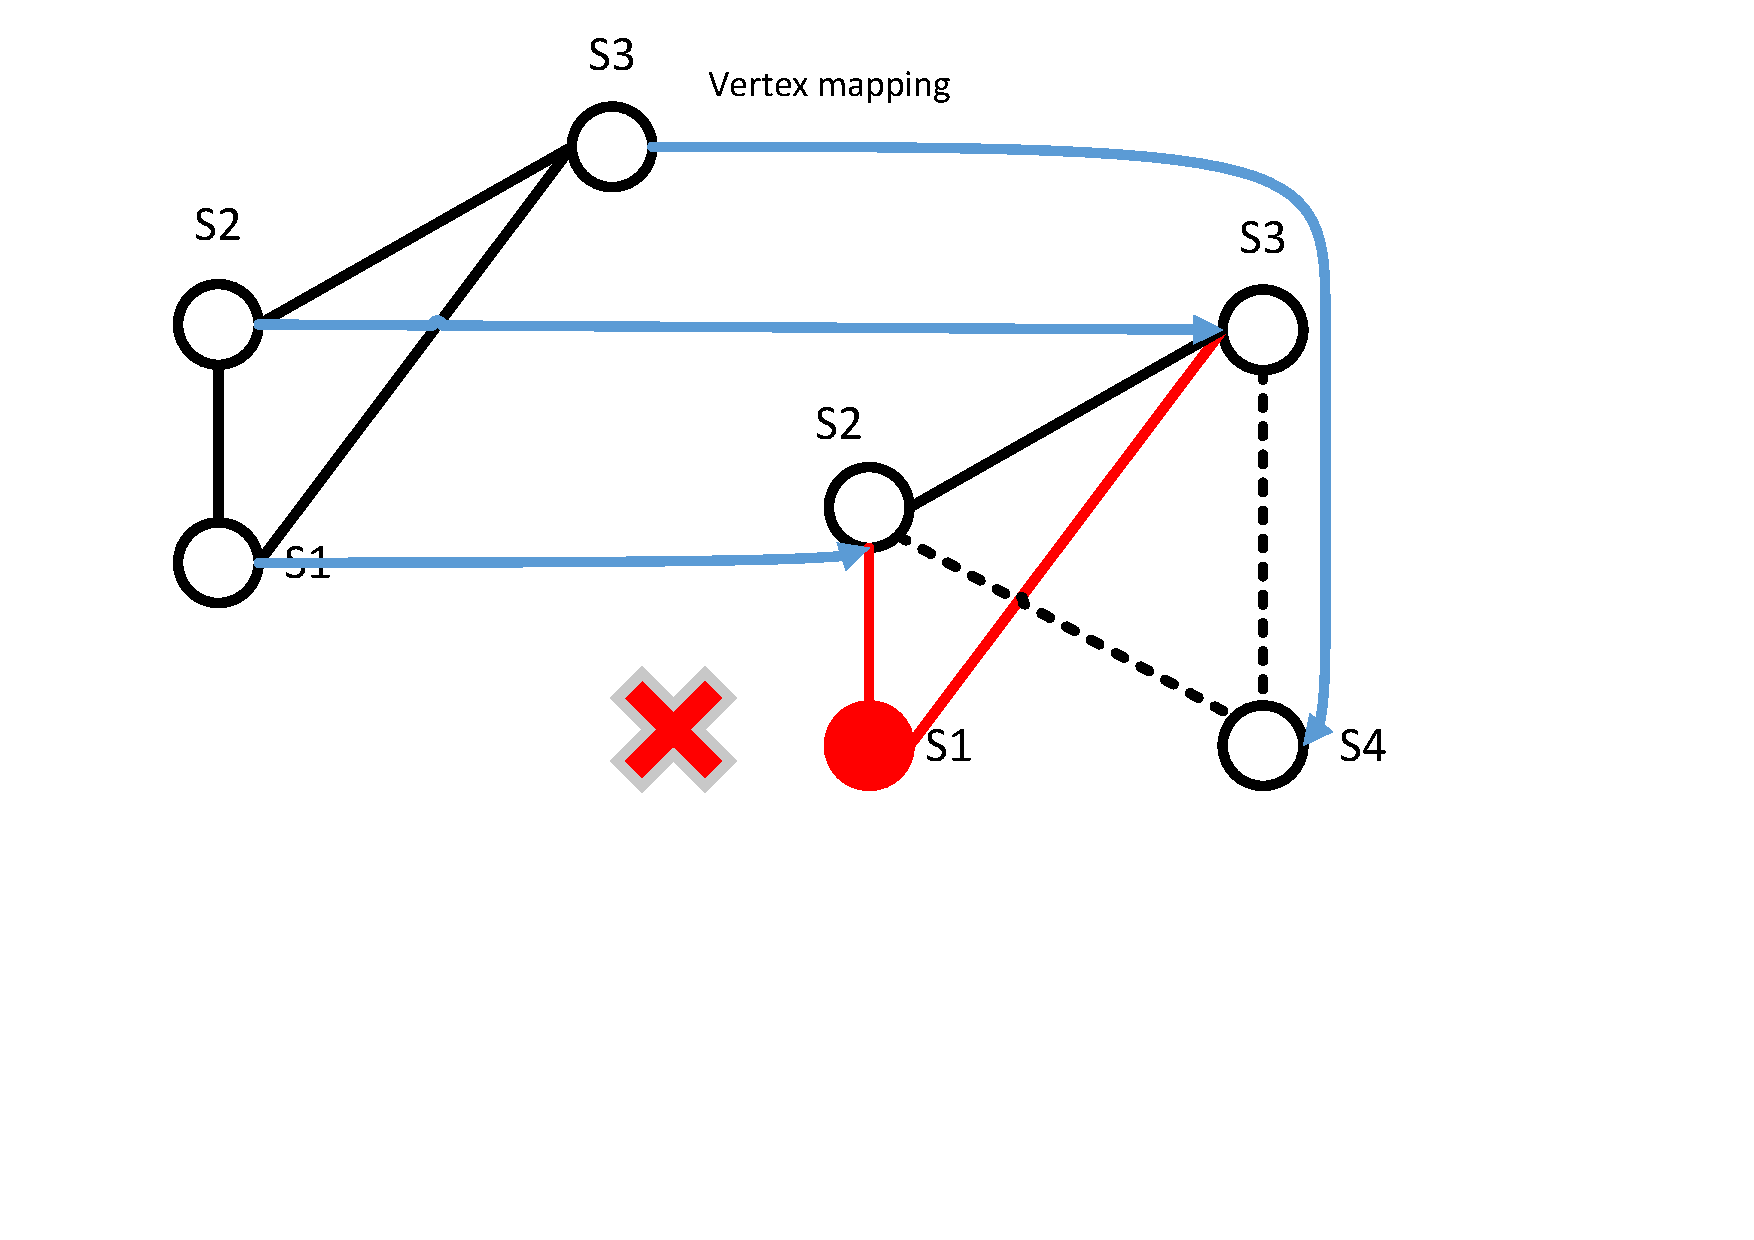
\includegraphics[width=1.5in]{Fig/MapB}\\
  \caption{MapB}\label{Fig:MapB}
\end{figure}



\begin{figure}
  \centering
  % Requires \usepackage{graphicx}
  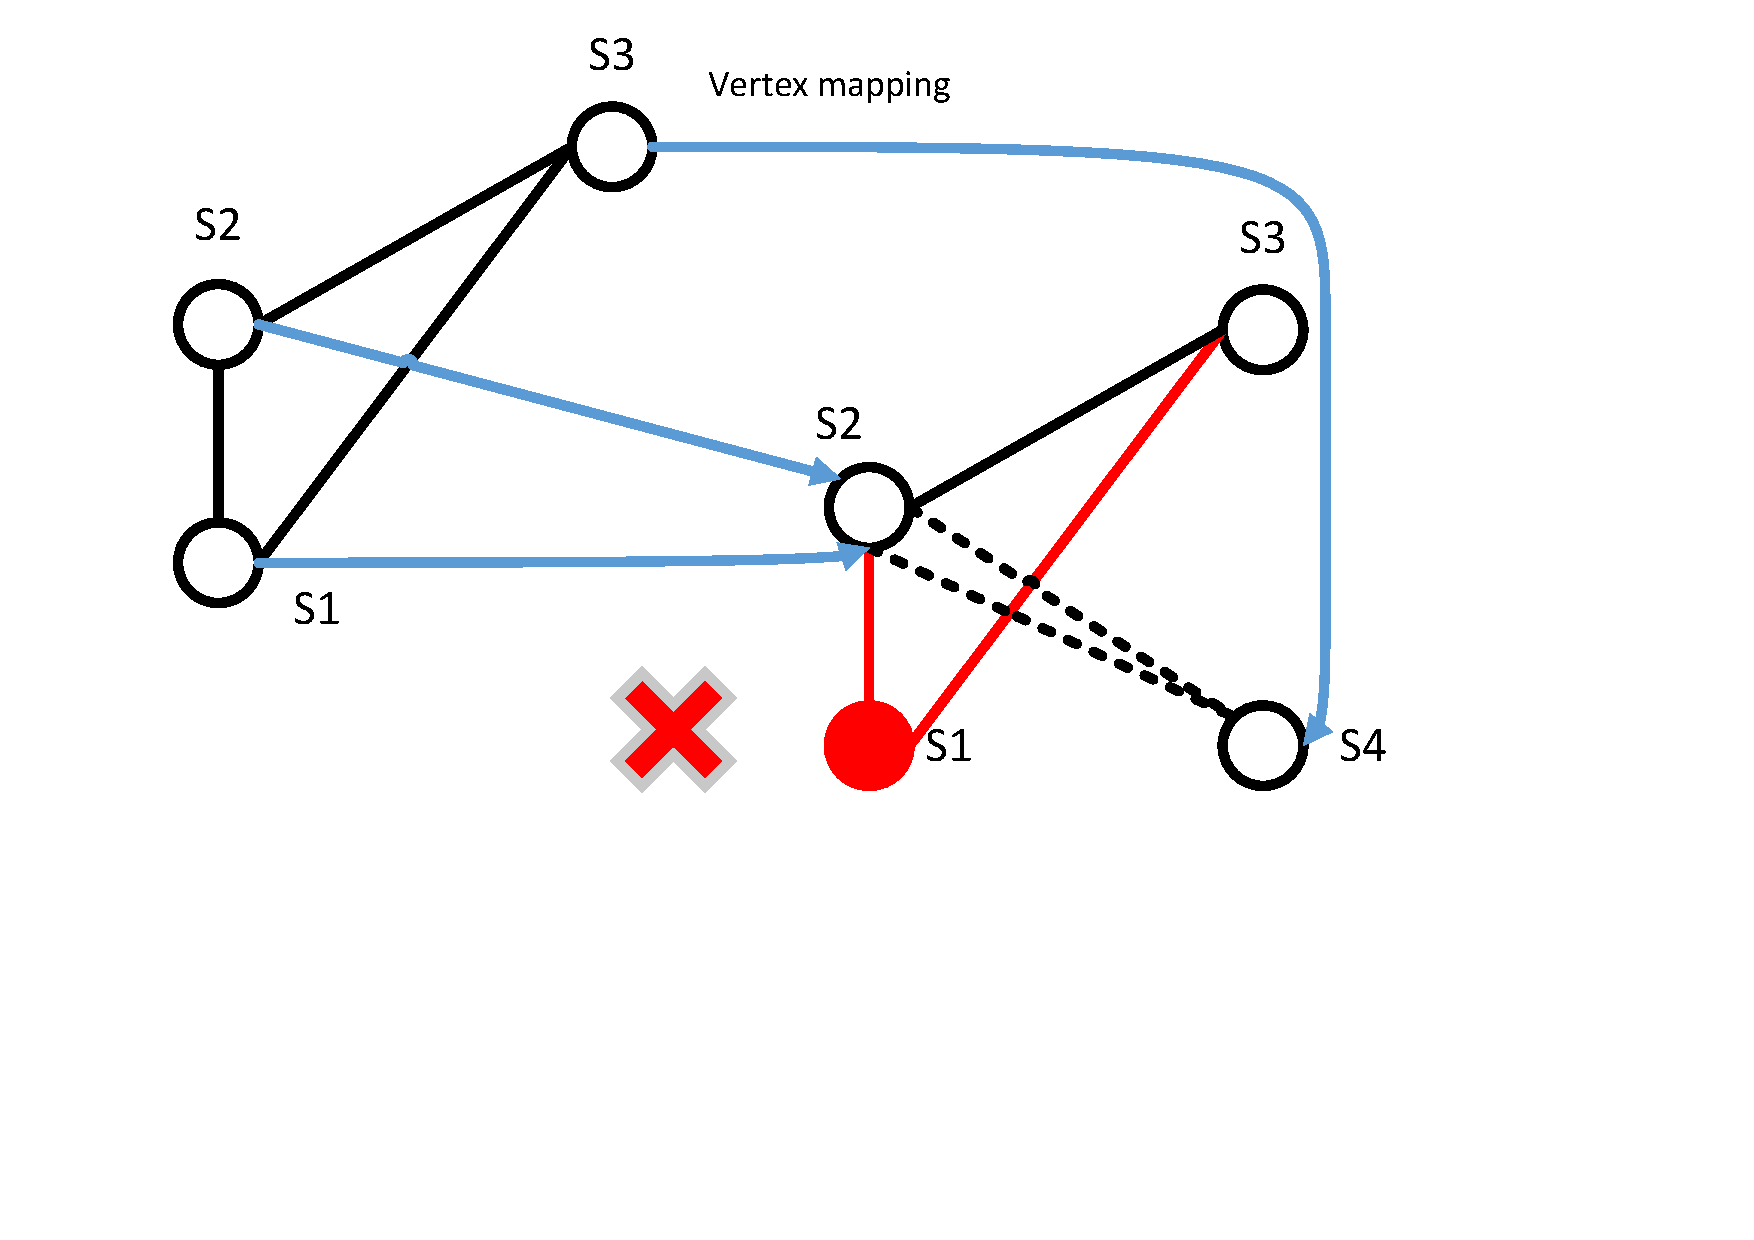
\includegraphics[width=1.5in]{Fig/MapC}\\
  \caption{MapC}\label{Fig:MapC}
\end{figure}

\begin{figure}
  \centering
  % Requires \usepackage{graphicx}
  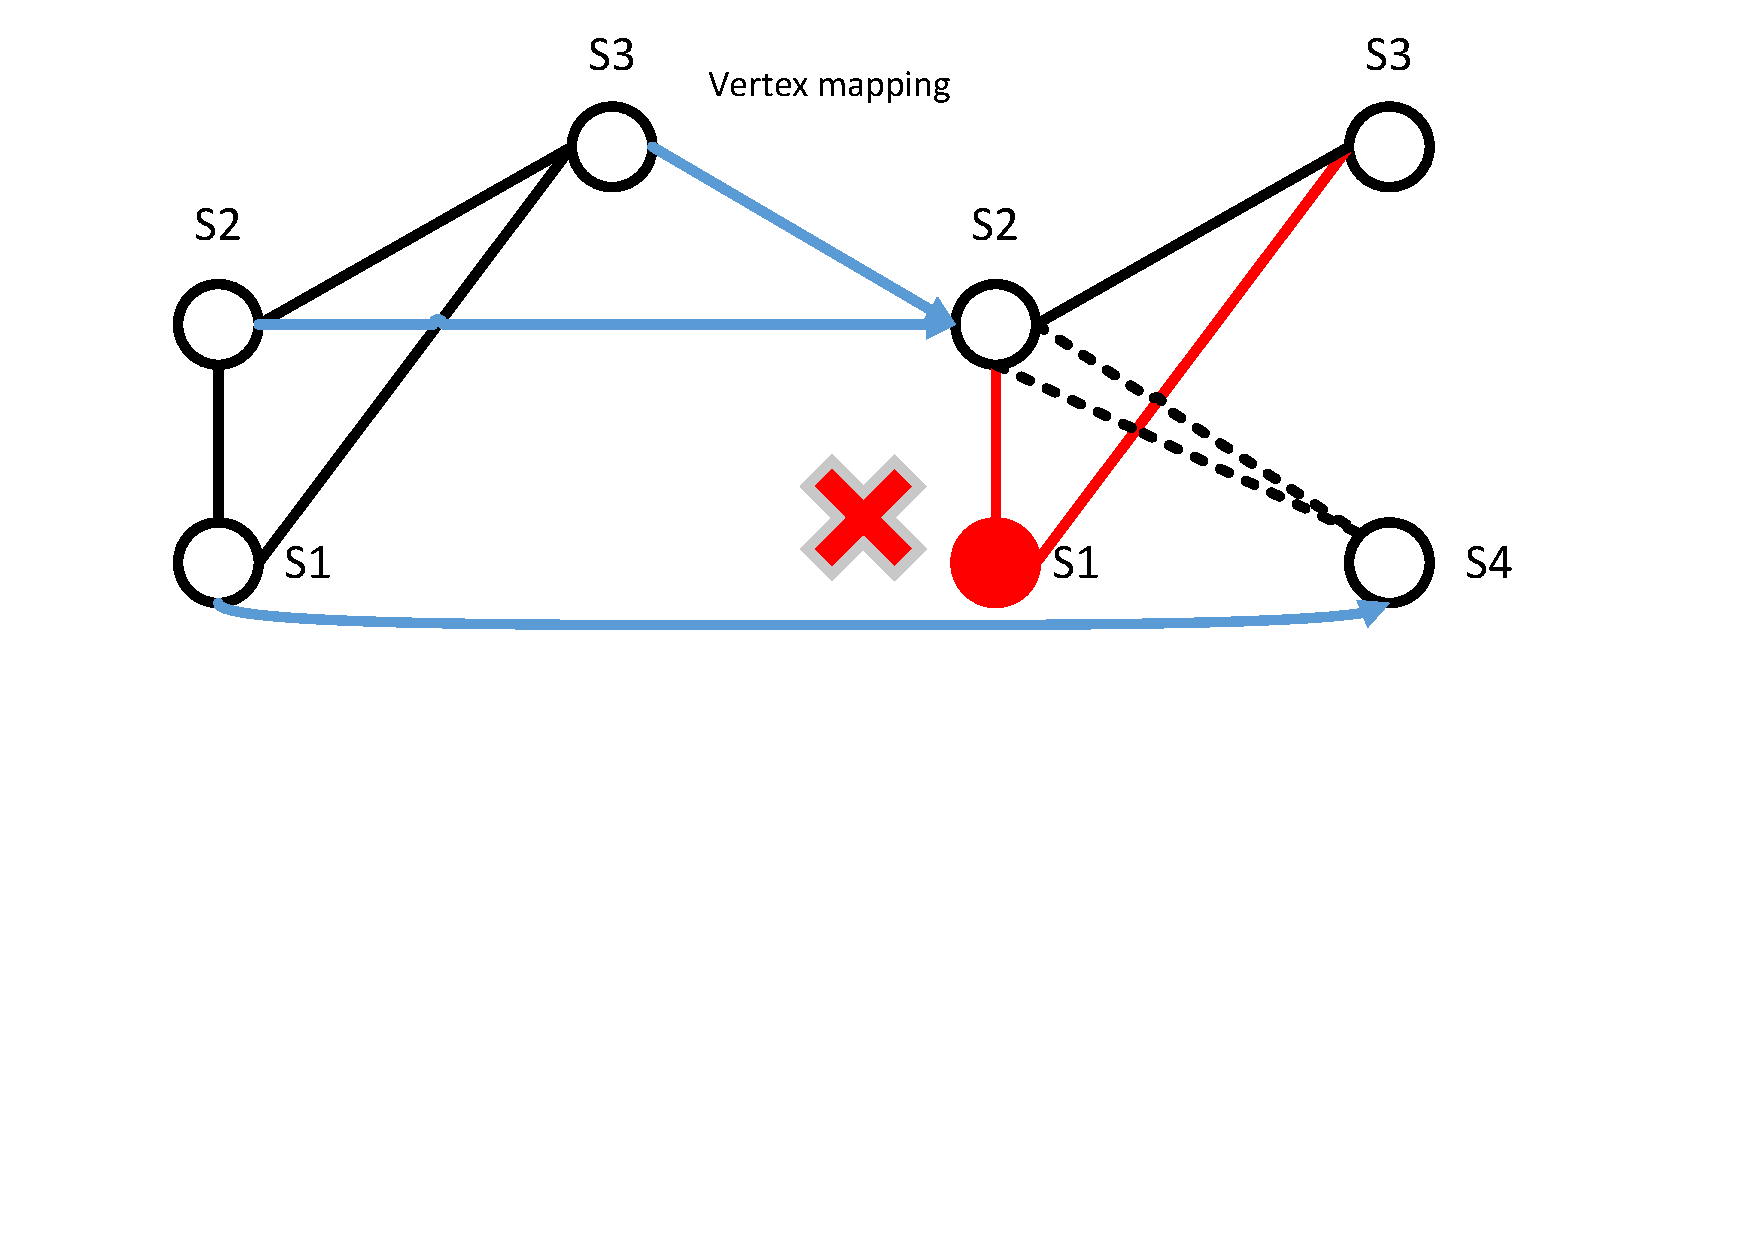
\includegraphics[width=1.5in]{Fig/MapD}\\
  \caption{MapD}\label{Fig:MapD}
\end{figure}


\begin{figure}
  \centering
  % Requires \usepackage{graphicx}
  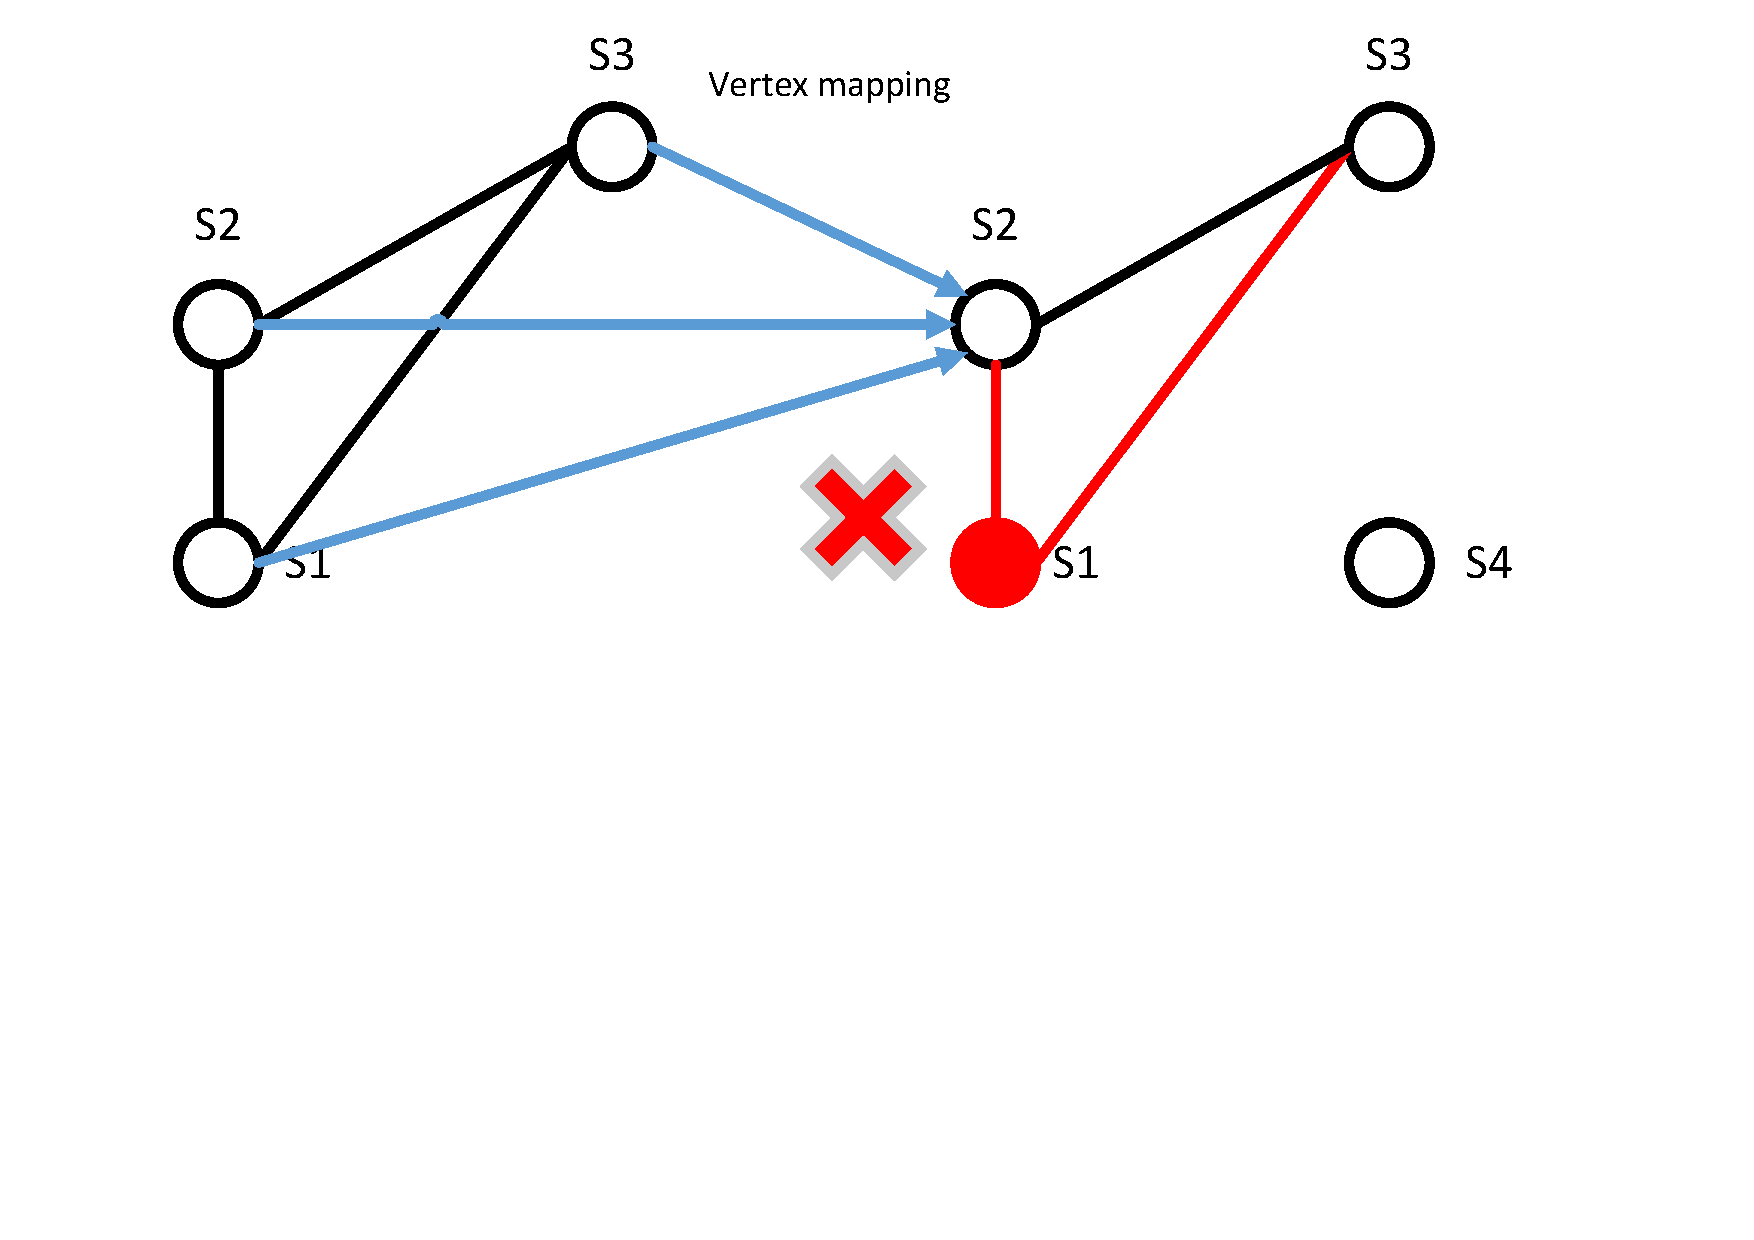
\includegraphics[width=1.5in]{Fig/MapE}\\
  \caption{MapE}\label{Fig:MapE}
\end{figure}
